\documentclass[tikz,14pt,fleqn]{article}

\setlength{\parskip}{0.5\baselineskip}%
\usepackage[utf8]{inputenc}
\usepackage[margin=1in]{geometry}
\usepackage[titletoc,title]{appendix}
\usepackage{latexsym}
\usepackage{amssymb}
\usepackage{gensymb}
\usepackage{amsmath}
\usepackage{amsfonts}
\usepackage[dvipsnames]{xcolor}
\usepackage{multicol}
\usepackage{graphicx}
\usepackage{fancyhdr}
\usepackage[linguistics]{forest}
\usepackage{colortbl}
\usepackage{pdfpages}
\usepackage{wrapfig}
\usepackage{cancel}
\usepackage{multirow}

\usepackage{minted}
\definecolor{LightGray}{gray}{0.95}
\setminted{
    frame=lines,
    framesep=2mm,
    baselinestretch=1.2,
    bgcolor=LightGray,
    fontsize=\small,
    linenos,
    mathescape=true,
    escapeinside=||,
}

\definecolor{darkblue}{rgb}{0.0, 0.0, 1}
\usepackage[pdftex,hyperfigures,hyperindex,bookmarksnumbered,colorlinks, bookmarks, breaklinks, linktocpage,citecolor=darkblue,urlcolor=darkblue,linkcolor=darkblue,pagebackref=true]{hyperref}
\usepackage{cleveref}

% to fixme
\usepackage{xcolor} 
\definecolor{FIXMECOLOR}{rgb}{1,0,0}
\newcommand{\FIXME}[1]{{\color{FIXMECOLOR}{\textbf{FIXME: #1}}}} 

% to simplify math 

\newcommand{\bvec}[1]{
   \ensuremath{
   \begin{bmatrix}
       #1 \\
   \end{bmatrix}
}}

\newcommand{\bmat}[1]{
   \ensuremath{
   \begin{bmatrix}
       #1
   \end{bmatrix}
}}

\newcommand{\dotprod}[2]{\ensuremath{\left< #1, #2 \right>}}

%% For plotting
\usepackage{pgfplots}
\pgfplotsset{width=10cm,compat=1.9}
\usepgfplotslibrary{external}
\tikzexternalize
%%
\usepackage{dirtree}
\usepackage{subcaption}
\usepackage{xifthen}% provides \isempty test
\usepackage{glossaries}

\captionsetup[subfigure]{labelformat=empty}
\definecolor{color1}{HTML}{0B0C10}
\definecolor{color2}{HTML}{1F2833}
\definecolor{color3}{HTML}{C5C6C7}
\definecolor{color4}{HTML}{66FCF1}
\definecolor{color5}{HTML}{45A29E}

\pagestyle{fancy}
\fancyhf{}
%%%%%%%%%%%%%%%%%%%%%%%%%%%%
%% VARIABLES
\newcommand\namesurname{Albert Cerfeda\\Alessandro Gobbetti}
\newcommand\assignment{Assignment 9}

\newcommand\subject{Computer Graphics}
\newcommand\documentdate{30.12.2022}

% Title content
%%%%%%%%%%%%%%%%%%%%%%%%%%%%
\rhead{\assignment}
\lhead{\namesurname}
%%%%%%%%%%%%%%%%%%%%%%%%%%%%
\rfoot{Page \thepage}
\setlength{\parindent}{0pt}

\newcommand\xdownarrow[1][2ex]{%
   \mathrel{\rotatebox{90}{$\xleftarrow{\rule{#1}{0pt}}$}}
}

\begin{document}

\begin{titlepage}
   \begin{center}
       \vspace*{0.2cm}

       \textbf{\Large{Rendering Competition}}

       \vspace{0.5cm}
        \textbf{\subject}\\[5mm]
       % \assignment
        
            
       \vspace{0.4cm}

        \namesurname
        \begin{figure}[H]
            \centering
            \includegraphics[width=0.9\linewidth]{fig/result.png}
        \end{figure}
       \tableofcontents

       \vspace*{\fill}
     
        \includegraphics[width=0.4\textwidth]{fig/logo.png}
       
        \documentdate \\
        Università della Svizzera italiana\\
        Faculty of Informatics\\
        Switzerland\\

   \end{center}
\end{titlepage}



\section{Introduction}
During the development of our raytracer, we always put a lot of effort into improving and maintaining a good rendering performance as the computational cost is the most apparent drawback of raytracing.

Apart from the usual good measures to reduce code complexity like storing parameters in constant variables when possible, and isolating recurrent computations, therefore, avoiding recomputing recurrent formulas, we went the extra mile namely by using thread-pooling and tiling.

We are overall quite satisfied with the current state of our raytracer.

Every object is either defined as a primitive or through a mesh of triangles, benefiting from performance improvements when using primitives but also with triangle meshes by using acceleration structures like \textit{bounding boxes}.

Texturing also allows for diverse approaches. We maintained the implementation of procedural textures and in addition, the raytracer has the ability to read the different maps from image files or by reading \verb|.obj| files. Regardless of the chosen texturing approach, the texture is abstracted into its own \verb|Texture| class.

One major aspect we wanted to improve was code modularity and separation. In the provided raytracer, all features and code were contained inside the \verb|main.cpp| file. We separated every section of the code into its own dedicated file for improved maintainability and readability.

We wanted to allow anyone to use our raytracer. Therefore we provided an easy to use \verb|Makefile| for rendering still renders and animations.

The code is available at:\\
\url{https://github.com/AlbertCerfeda/ComputerGraphics/tree/main/RenderingCompetition}.




\section{Features}

\subsection{Texturing}
Textures are fundamental when defining a 3D scene. Textures try to imitate surface properties like color, roughness, and how light interacts with the surface. Texturing the objects in the scene can result in an increase in realism and immersion.

Textures are composed of multiple 'layers' or maps each defining a surface property:
\begin{figure}[h!]
\centering
\includegraphics[width=0.6\linewidth]{fig/maps.png}
\caption{Different maps of which a texture is composed of}
\end{figure}

Our raytracer supports different kinds of textures:
\begin{itemize}
    \item \textbf{Procedural textures}\\
    These textures are defined as functions that take as parameters the \verb|(x,y)| coordinates in the texture. A clear example of this type of texture is the \textit{checkerboard} texture.
    \begin{minted}{cpp}
    inline glm::vec3 checkerboardTexture(glm::vec2 uv) {
        int n = 30;
        return glm::vec3(abs(int(floor(n * uv.x) + floor(n * uv.y)) % 2));
    };
    \end{minted}
    \item \textbf{Textures from image files}\\
    When defining a texture our raytracer allows us to pass the path to an image map on our filesystem. This allows us to also load textures downloaded from the internet, like so:
    \begin{minted}{cpp}
    Material fur;
    fur.setDiffuse("src/Textures/fur_basecolor.jpg");
    fur.setAmbient("src/Textures/fur_ambientOcclusion.jpg");
    fur.setRoughness("src/Textures/fur_roughness.jpg");
    fur.setNormal("src/Textures/fur_normal.jpg");
    \end{minted}
    \begin{figure}[h!]
        \centering
        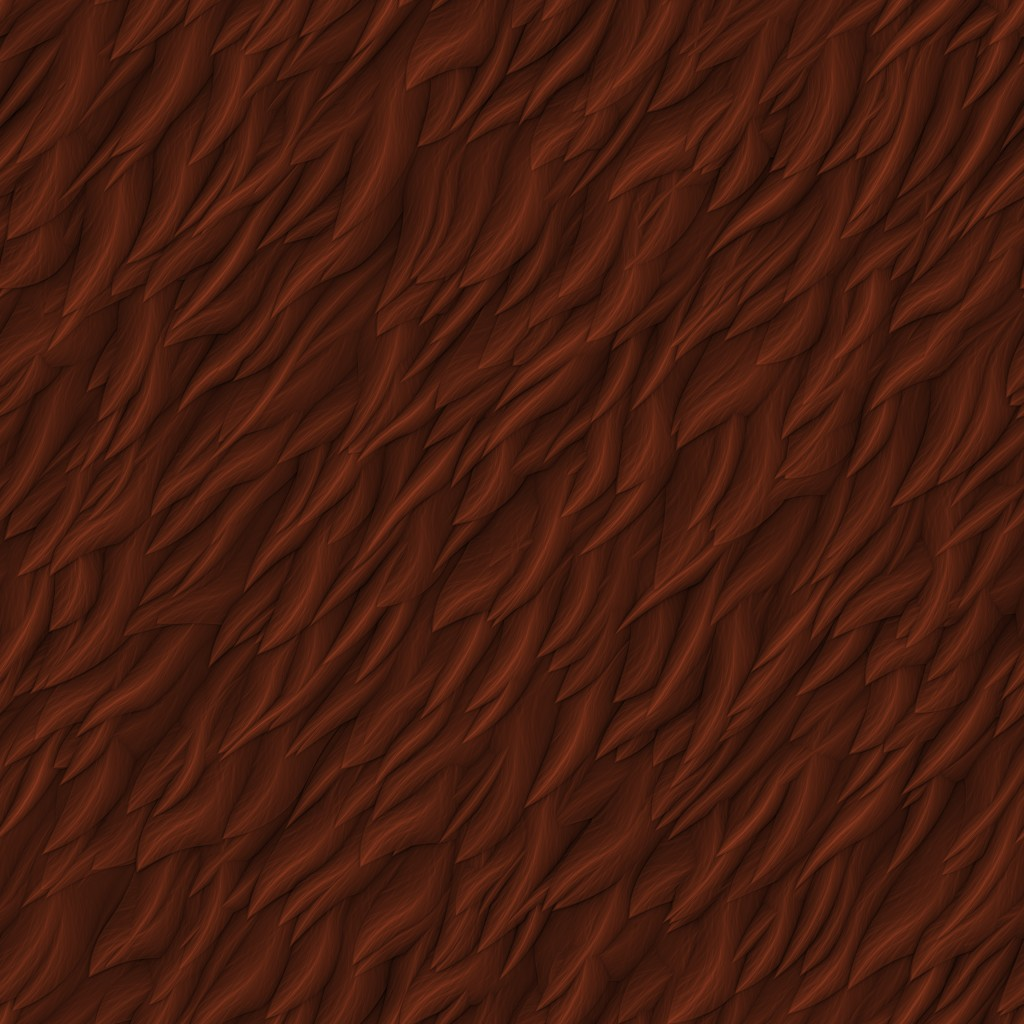
\includegraphics[width=0.24\linewidth]{fig/fur_basecolor.jpg}
        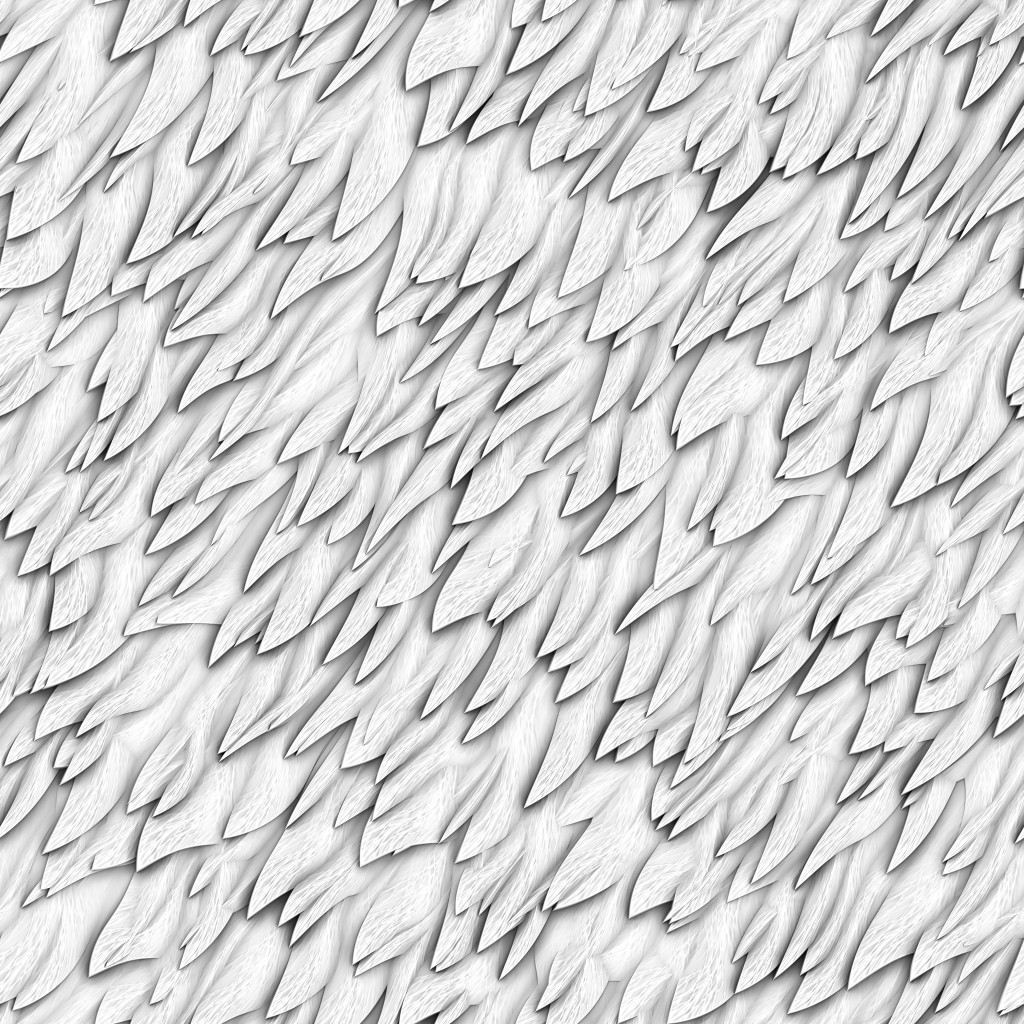
\includegraphics[width=0.24\linewidth]{fig/fur_ambientOcclusion.jpg}
        
\includegraphics[width=0.24\linewidth]{fig/fur_roughness.jpg}
        
\includegraphics[width=0.24\linewidth]{fig/fur_normal.jpg}
        \caption{The \textit{fur} texture}
    \end{figure}
    
    \item{\textbf{Textures from \textit{.mtl} files}}\\
    When loading a scene through an \verb|.obj| file, the textures get also loaded from the relative \verb|.mtl| file.
\end{itemize}

\subsection{Meshes \& Acceleration Structure}
A good render engine must be used with external objects modeled by the user. So far we have only used spheres, cones, and planes, but creating a scene with only these objects is not very interesting.
This section will discuss how to handle triangle meshes, how to accelerate the intersection tests with them, and how to load external obj files into our scene.

\subsubsection{Triangle Soups}

In order to render complex scenes we need to be able to handle triangles, since the more complex objects may be approximated by triangles.





A scene may be made of multiple triangles, not necessarily connected to each other: these are called triangle soups.
For each triangle soup, we maintain a material array and an array of triangles. 

\begin{minted}{cpp}
class TriangleSoup : public Object {
   protected:
    vector<Material> materials;
    vector<Triangle> triangles;
    |\vdots|
}
\end{minted}

Each triangle stores the 3 vertices' positions, normals, texture coordinates, and an index in the material table.   

\begin{minted}{cpp}
class Triangle {
   public:
    glm::vec3 p[3];
    glm::vec3 n[3];
    glm::vec2 uv[3];
    int material_index;
    |\vdots|
}
\end{minted}

To compute the intersection between the ray and the triangle we use the \href{https://en.wikipedia.org/wiki/M%C3%B6ller%E2%80%93Trumbore_intersection_algorithm}{Möller–Trumbore} method, 
that computes from the three vertex coordinates the barycentric coordinates of the ray intersection and checks whether they are inside the triangle. If an intersection exists the barycentric coordinates are used to interpolate normals and texture coordinates at the intersection point.

In order to get a nice intersection, we consider rays nearly parallel to the triangle plain not intersecting (otherwise, the error is too big to trust the intersection).
By setting the \mintinline{cpp}{cull_backfaces} parameter to \mintinline{cpp}{true} we can also ignore the intersections if the triangle is not facing the ray.

\subsubsection{Axis-Aligned Bounding Boxes (AABBs)}
A scene may involve thousands or millions of triangles and when shooting a ray we need to check the intersections with every object in the scene. We thus need to find an efficient way to do so.
The method we use is to hierarchically aggregate nearby scene portions, compute bounding volumes for each portion and check intersections by descending in the hierarchy so as to quickly skip portions of the scene far from the ray.

The specific acceleration structure that we use is the Axis-Aligned Bounding Box Tree. Each node in the tree contains a bounding box of the scene portion associated with it. The inner nodes contain two references to child nodes, while the leaf nodes contain the list of triangles. 

During the tree construction, the triangles in the soup are re-ordered so as to contiguously store the triangles in each leaf node. This way a leaf node needs only to store the index of the first triangle and the count.

\begin{minted}{cpp}
class AABoxTreeNode {
   public:
    AABox bounding_box;

    // For leafs
    int leaf_triangle_count;
    int leaf_first_triangle;

    // For inner nodes
    int left_index;
    int right_index;
    |\vdots|
}
\end{minted}

The tree construction routine works recursively: if the number of triangles is less than a threshold a leaf node is created, otherwise, the list of triangles is split into two halves, each half is assigned to an inner node and the construction continues recursively.

The bounding box associated with each node is the smallest one containing all the triangles: it is created by adding all vertices and adapting the minimum and maximum coordinates of the box.
In order to avoid degenerate cases during the ray intersection, we also expand the boxes by a small amount ($1e-6$), so that we avoid returning no intersection for flat boxes.

To split the triangles list into halves, the centroids of the triangles are considered. We first compute a bounding box of all the centroids, we determine the longest axis, and the box is split by a plane orthogonal to it and passing through the box center.
The reasoning behind splitting along the longest axis is to better geometrically subdivide the space, this way we obtain more 'cubic' boxes rather than stretched ones.

The triangles are partitioned according to the placement of their centroids with respect to the plane.

When shooting a ray, we recursively test intersections with the bounding box tree nodes starting from the root. At each node, we first check the intersection with the bounding box. If no intersection is found, no other computation is needed. If instead, an intersection exists, if the node is a leaf we test the intersection with all the triangles, and store the closest to the origin of the ray between the current one and the best found. If the node is an inner one, we recursively compute the intersection for both children and keep the closest one. 

Note that the structure does not partition the space, and the bounding boxes of children may overlap. This is because we do not clip the triangles when we distribute them into child nodes at construction time. 


We made some tests to verify the effectiveness of this acceleration structure. The graph in \autoref{fig:barplot} shows time to build the AABB tree and to render a $1000\times 1000$ image of the 'kitchen' scene for a number of triangles per leaf ranging from 2 and 256. The scene contains 270 634 triangles. The table in \autoref{tab:benchmark} presents the same data but also includes the case where no acceleration structure is provided.

\begin{table}[H]
    \centering
    \begin{tabular}{|r|r|r|}
        \hline
        \textbf{Triangles per leaf} & \textbf{Time to build AABB tree} & \textbf{Time render}\\
        \hline
        2 & 0.128621 & 1.24209  \\
        4 & 0.105007 & 1.09056 \\
        8 & 0.096488 & 1.07354 \\
        16 & 0.090599 & 1.17396 \\
        32 & 0.085605 & 1.35231 \\
        64 & 0.080311 & 1.71468 \\
        128 & 0.077422 & 2.26410 \\
        256 & 0.072714 & 3.15491 \\
        $\infty$ & 0		   & 1738.49 \\
        \hline
    \end{tabular}
    \caption{Time to build AABB tree and time to render for different number of triangles per leaf}
    \label{tab:benchmark}
\end{table}

\begin{figure}[H]
    \centering
    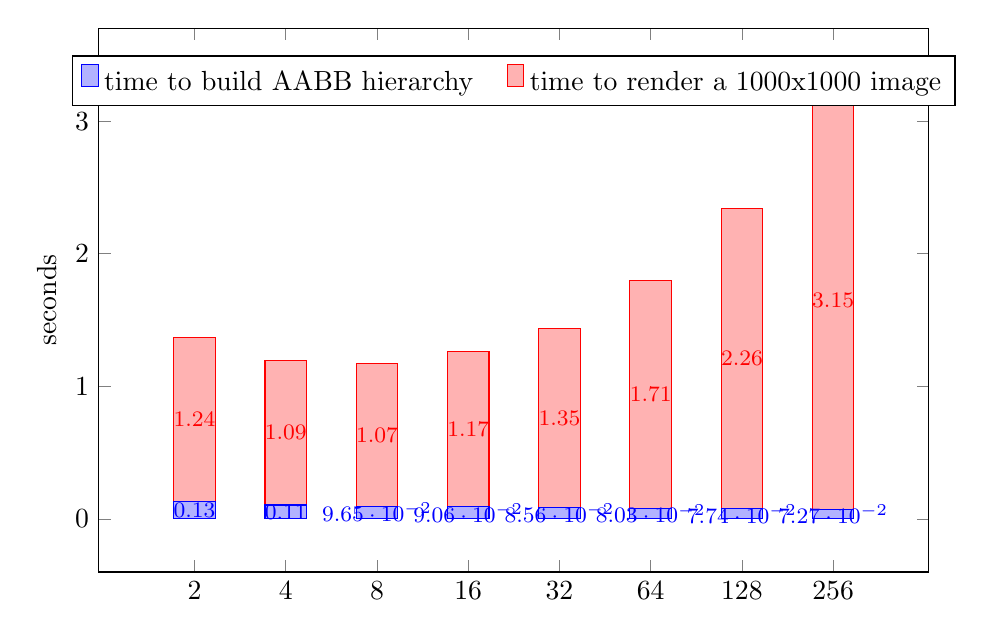
\begin{tikzpicture}
        \centering
        \begin{axis}[
        ybar stacked,
        width=\linewidth,
        height=0.7\linewidth,
        bar width=15pt,
        nodes near coords,
        enlargelimits=0.15,
        legend style={at={(0.5,0.95)},
        anchor=north,legend columns=-1},
        ylabel={seconds},
        symbolic x coords={2, 4, 8, 16, 32, 64, 128, 256},
        xtick=data,
        every node near coord/.append style={font=\footnotesize},
        ]
    \addplot+[ybar] plot coordinates {(2, 0.128621) (4, 0.105007) 
      (8, 0.096488) (16, 0.090599) (32, 0.085605) (64, 0.080311) (128, 0.077422) (256, 0.072714)};
    \addplot+[ybar] plot coordinates {(2, 1.24209) (4, 1.09056) 
      (8, 1.07354) (16, 1.17396) (32, 1.35231) (64, 1.71468) (128, 2.26410) (256, 3.15491)};
    \legend{\strut time to build AABB hierarchy\quad\quad, \strut time to render a 1000x1000 image}
    \end{axis}
    \end{tikzpicture}
    \caption{Benchmarks to find best AABB hierarchy}
    \label{fig:barplot}
\end{figure}





As you can see in \autoref{tab:benchmark} and \autoref{fig:barplot}, the
time to build the AABB tree is very little with respect to image rendering time, 
but the structure is very effective in reducing rendering time.

On my machine, the optimal granularity is around 8 triangles per leaf, with no significant change until 32 triangles per leaf.
Without acceleration structure (or only one box that contains the whole triangle soup),
the time to render is 1738.49 seconds (28 minutes and 58 seconds), while in the best conditions the render is done in almost 1 second: over 1600 times faster!


\subsubsection{Load OBJ files}
As well as we load images with the \texttt{stb\_image} library, to load the OBJ files, we use the \texttt{tinyobjloader} library, which is a single-file C++ library for loading OBJ files.
The library is very easy to use, and it is very fast.

Once the objects are loaded from the OBJ files, we have to convert the data structure used by the library to our own data structure, which is the triangle soup of triangles, and a list of materials we load from the \texttt{.mtl} file.
If smooth shading is enabled the normals at vertices are recomputed as the average of the normals of the incident triangles. We directly used the code provided with the \texttt{tinyobjloader} viewer to perform the operation.

If the scene is successfully loaded, we build the bounding box hierarchy for the triangles.

\subsection{Optimizations}
As stated in the introduction, we put particular effort into making the raytracer as efficient as possible.
\subsubsection{Compiler Optimizations}
The first step that was taken was by introducing compiler optimization flags. GCC allows the use of many optimization flags to be passed at compile time. GCC has different \textit{optimization levels} that can be enabled: \verb|-O1|, \verb|-O2|, \verb|-O3|, \verb|-Ofast| ecc. Each level enables further optimizations than the previous levels. We went with optimization level \verb|O3|, as the \verb|Ofast| level disables strict standards compliance and allows for data races. Nevertheless, the use of the \verb|-O3| compiler flag leads to noticeable performance improvements.



\subsubsection{Thread pools and tiling}
The final optimization step taken was to implement thread-pooling and tiling.

The main advantage with thread-pooling over simple multithreading is that with multithreading a fixed number of threads is created and each thread executes one job and then gets terminated and deallocated from memory. Therefore, for every job a thread needs to be specifically created and then destroyed once the thread has finished executing its job.

This results in significant performance overhead coming from the repetitive creation and destruction of threads. Thread pools solve this issue by having a job queue and assigning them to free threads. The same threads, once they have finished their task, check again into the job queue and if there are any, take new tasks to execute.

The OpenMP standard aims to standardize multi-language high-level parallelism. GCCs implementation can be activated by using the \verb|-fopenmp| compiler flag. A very neat feature we used in our raytracer is the ability to automatically parallelize loops, like so:
\begin{minted}{cpp}
#pragma omp parallel for schedule(dynamic, 1)
for (int tile = 0; tile < tile_count; tile++) {
    // ...
}
\end{minted}
By adding the \mintinline{cpp}{#pragma} compiler annotation we instruct the compiler to assign each iteration of the for loop to a separate thread. By specifying \mintinline{cpp}{schedule(dynamic,1)} we tell GCC to assign a new job to a thread once it has finished executing its current one, instead of destroying it and creating a new one.

\textit{Tiled rendering} is the process of dividing the frame into sub-frames called \textit{tiles}. This approach is opposed to the classic one of rendering the whole frame at once. The main benefits are regarding memory bandwidth, as once each tile is rendered it can be separately stored on disk, without requiring the whole frame to be in RAM at once.

In our raytracer we divide the frame into separate tiles, and assign the rendering of each one of them to a separate thread, using GCC's OpenMP implementation.

These tweaks lead to pretty significant performance improvements. It is worth mentioning that the tile size influences render time as shown by the table below:


\begin{table}[h!]
    \centering
    \begin{tabular}{c|c}
        Tiles size (px) & Render time (seconds)\\ \hline
        $8\times 8$ &  1.17342\\
        $16\times 16$ &1.17348\\
        $32\times 32$ &1.18070\\
        $64\times 64$ &1.19527\\
        $128\times 128$ & 1.23983\\
        $256 \times 256$ & 1.45017\\
        $512 \times 512$ & 2.31396\\
        $1024 \times 1024$ & 7.13384
    \end{tabular}
    \caption{Render time in regards to tile sizes for a $1000\times 1000$ pixels image of the 'kitchen' scene on a 12-core machine.}
\end{table}
In general, it can be advised to divide the scene in tiles \textit{at least} the same amount as the number of cores of the CPU, as we ensure that no threads are \textbf{idling}. As the number of tiles grows, the performance overhead from assigning each tile to a new thread in the pool starts to negatively impact our render time.

Other various optimizations are also present in the code.

\subsection{Anti-Aliasing}
When an image is displayed on a screen, the pixels that make up the image can sometimes create a staircase effect, known as "aliasing," along the edges of objects. 
This can make the image look pixelated or blocky.

Anti-aliasing is a technique used to reduce the jagged edges of the rendered image.
The idea is to shoot multiple rays for each pixel, and then average the colors of the intersections.
Since anti-aliasing involves shooting more rays, it slows down the rendering process.
Shooting too many rays may not be worth it, since the contribution of each ray is very small compared to the added rendering time, while shooting too few rays may not be enough to reduce the aliasing effect.

Our implementation of anti-aliasing is very simple: we shoot $n$ rays for each pixel, and then we average the colors of the intersections. 
The pixel is subdivided into a grid of $n$ sub-pixels, and we shoot a ray in a random position in each sub-pixel.


\begin{figure}[H]
    \centering
    \begin{tabular}{ccc}
    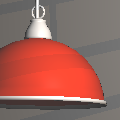
\includegraphics[width=0.3\textwidth]{fig/anti-aliasing-OFF.png} & 
    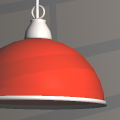
\includegraphics[width=0.3\textwidth]{fig/anti-aliasing-ON.png} &
    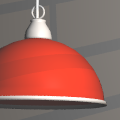
\includegraphics[width=0.3\textwidth]{fig/anti-aliasing-ON-jittered.png} \\
    \textbf{Anti-Aliasing OFF} & \textbf{Anti-Aliasing ON} & \textbf{Anti-Aliasing ON + jitter}  \\
    \end{tabular}
    \caption{Anti-Aliasing effect}
    \label{fig:antialiasing}
\end{figure}


In \autoref{fig:antialiasing}, we show the effect of anti-aliasing on a detail of the 'kitchen' scene.
The left image is rendered without anti-aliasing, it is clearly visible the stair effect.
The image in the middle is rendered with anti-aliasing but without randomizing the position of the rays: each ray is shot in the middle of the sub-pixel.
The stair effect is less visible but still present.
On the right, we show the result of anti-aliasing with randomization. Our mind is sensible to linear patterns, and the randomization of the rays makes the stair effect less visible and more natural.
The images with anti-aliasing are rendered with $3*3$ rays per pixel.




\end{document}